\documentclass[11pt]{article}
\usepackage{latexsym}
\usepackage{hyperref}
\usepackage{listings}
\usepackage{color}
\usepackage{geometry}


\usepackage{titling}
% \renewcommand\maketitlehooka{\null\mbox{}\vfill}
\renewcommand\maketitlehookd{\vfill\null}

\geometry{a4paper, margin=1in}
\usepackage{natbib}  % Added for citation management

\usepackage{graphicx}
\graphicspath{./images}

\begin{document}
\begin{titlepage}
    \title{
\includegraphics[width=7cm]{./images/swinburne}\\Intelligent System \\ Assignment 1 - Option B \\ Applying Macroeconomic Indicators to Predict Stock Prices}
    \author{Xuan Tuan Minh Nguyen - 103819212}
    \date{\today}
\end{titlepage}

\begin{titlingpage}
    \maketitle
\end{titlingpage}


\pagebreak

\tableofcontents

\newpage

\begin{abstract}
   The major purpose of this research is to showcase \textbf{the application of
   machine learning} in predicting stock prices with the combination of \textbf{historical}
   data of \textbf{Macroeconomic Indicators}. In this research, we will focusing on researching
   the affect of the \textbf{Macroeconomic Indicators} to the stock price prediction.
   We will be using two most popular models for time series prediction, which are
   the \textbf{XGBoost} and \textbf{RandomForest} models. In addition, the stock price data will be taken
   from \textbf{Yahoo Finance}, and the Macroeconomic Indicator data will be taken from
   \textbf{FRED}. The research will be conducted on \textbf{Tesla Inc.} (TSLA) stock from the date of 2015-01-01 to 2023-08-25.
   This research will deep dive into \textbf{differentiating} each \textbf{potential solutions} to improve the
   performance of the \textbf{v0.5} codebase, \textbf{pick and implement} the solution that fits the most for the context.
   And \textbf{visualize} the \textbf{prediction results} with the actual stock prices to evaluate the performance of the models.
\end{abstract}


\section{Introduction}
With the significant development of the stock market, more and more investors are interested in
pouring their money into the stock market to gain profits. However, with the unpredictable nature
of the stock market, it is very difficult for investors to see when is the perfect time to buy or
sell their stocks. Therefore, with the phenomenon growth of the \textbf{machine learning} field,
investors could empower the \textbf{machine learning} to predict the future direction of the stock
market and could make their own decisions based on the predicted results.

In this research, we will be exploring the application of \textbf{machine learning} in the context of
predicting the stock prices. Stock price prediction could be a very complicated task as there are multiple
factors to consider, such as the \textbf{fundamental analysis} and \textbf{technical analysis}. In this research,
we will be analyzing the potential solutions to improve the performance of the \textbf{v0.5} model, which itself
strongly relies on the \textbf{historical stock prices} and have a bad performance in the prediction accuracy.
After that, we will be discussing and picking the best solution to give our \textbf{v0.5} an update to \textbf{v0.6},
which has a better and more reliable prediction accuracy.

\section{Review of the Potential Solutions}
Nowadays, there are multiple different approaches that have been proposed to improve the performance of the traditional
stock price prediction models. These approaches aimed for increase the accuracy and broaden the scope of the prediction
features by adding more data sources to the model, extending the modeling and data processing techniques and inputting
external factors that could affect the stock prices. These solutions could be categorized into:

\subsection{Improving the current Ensemble Prediction Model}
To improve the current ensemble prediction model, using an ensemble of multiple models could be a good solution. Two key
approaches that could be used to improve the performance of the ensemble prediction model are:
\begin{itemize}
    \item \textbf{Stacking Ensemble}: With the powerful non-linear nature of the stacking ensemble, which allows it to
    combine the predictions from multiple models to create a new model that has a better performance than the individual models,
    we could use the stacking ensemble to ensemble the predictions from the state of the are
    models, such as \textbf{Random Forest} and \textbf{XGBoost} models, to achieve a higher preidction accuracy and reducing the
    generalization error. \cite{Jiang2020-xl}
    \item \textbf{Bagging / Boosting Ensemble}: In addtion to the stacking ensemble, the Bagging and Boosting are the two most popular
    ensemble methods to improve the performance of the prediction model. The bagging ensemble method is used to reduce the variance of the prediction model,
    while the boosting ensemble method is used to reduce the bias of the prediction model. Thus could help to improve the prediction accuracy and reducing the
    generalization error. \cite{Jiang2020-xl}
\end{itemize}

\subsection{News and Social Media Content}
The sentiment of a market could strongly affect the stock prices, as the sentiment of the market could affect the behavior of the investors,
which in turn could affect the stock prices. Therefore, with the development of the \textbf{natural language processing} field, more and more
research aimed to use the sentiment analysis to predict the future direction of the stock prices. The following methods were explored:
\begin{itemize}
    \item \textbf{News and Social Media Content}: By collecting the news and social media content, we could use the sentiment analysis to predict the future direction of the stock prices, like what \cite{Bharathi2018-qx} did.
    \item \textbf{Sentiment Analysis}: Natural Language Processing (NLP) is a field that focuses on the interaction between computers and humans using natural language. With the development of the NLP field,
    we could use the sentiment analysis to predict the future direction of the stock prices, which could result in a higher accuracy. \cite{Bharathi2018-qx}
\end{itemize}

\subsection{Macroeconomic Indicators}
It is a well-known fact that some macroeconomic indicators could have a strong correlation with the stock prices, such as the \textbf{unemployment rate} and \textbf{inflation rate} \cite{Haque2023-kt}.
The following methods were found to be effective in predicting the stock prices:
\begin{itemize}
    \item \textbf{Inclusion of Macroeconomic Indicators}: Beside from the stock-specific data, such as the open, close, high and low prices, the volume of the stocks traded and the adjusted close price,
    we could include the macroeconomic indicators that have a strong correlation with the stock prices to improve the prediction accuracy, such as \textbf{GDP}, \textbf{inflation rate} and \textbf{unemployment rate}. \cite{Haque2023-kt}
    \item \textbf{Technical Indicators}: By adding technical indicators, such as \textbf{RSI}, \textbf{MACD} and \textbf{William Percent Range}, we could see the overbought and oversold levels on a chart and can
    help predict where a price is likely to go next, based on past performance. \cite{Cutkovic_undated-fh}
\end{itemize}

\subsection{Advanced Model Optimization Techniques}
Different optimization techniques are researched and have been widely used for improving the performance of the prediction model, such as:
\begin{itemize}
    \item \textbf{Hyperparameter Optimization}: By finding the optimal hyperparameters for the model, we could improve the prediction accuracy and reducing the generalization error. \cite{Bergstra2012-gr}
    \item \textbf{Random Search}: Random search is a technique that randomly samples a set of hyperparameters from a given distribution and then evaluates the performance of the model with those hyperparameters.
    This technique can help to find the optimal hyperparameters for the model, which could improve the prediction accuracy and reducing the generalization error. \cite{Bergstra2012-gr}
    \item \textbf{Early Stopping and Learning Rate Scheduling}: Early stopping is a technique that stops the training process when the performance of the model starts to decrease, which could help to prevent overfitting.
    Learning rate scheduling is a technique that adjusts the learning rate during the training process, which could help to increase the prediction accuracy and reducing the error.
\end{itemize}

\subsection{Advanced Model Applications}
Moreover, there are some advanced applications that could be used to improve the performance of the prediction model, such as:
\begin{itemize}
   \item \textbf{Deep Reinforcement Learning}: Deep Reinforcement Learning (DRL) allows agents to learn directly from raw sensory input, such as images or sounds, without relying on handcrafted features or domain-specific knowledge.
   Thus making DRL highly flexible and capable of automating tasks, including stock trading. \cite{Khan2023-zu}
   \item \textbf{Time series Analysis}: Using time-series based models, such as \textbf{ARIMA}, we could effectively predict the short-term stock price and stock returns movements, thanks to the ability of time-series models to
   capture the underlying patterns and trends in the data. \cite{Hardikkumar2021-ry}
\end{itemize}
\section{Implementation}
After carefully reviewing and considering the researched potential approaches, I have decided to go with the \textbf{Macroeconomic Indicators} approach, as it has a strong correlation with the stock prices, has a high compatibility with the current v0.5 codebase, and has a good prediction accuracy.
In addition, the \textbf{Macroeconomic Indicators} approach could give me a good point of view to how the macroeconomic indicators could affect the stock prices and how we could use it for the prediction.
\subsection{Environment Setup}
\subsubsection{Create a new environment using Conda CLI}
There are several different procedures to create an environment, but the given procedure below will encapsulate all of the required steps to create a safe and clean environment using Conda \citep{Nti2019-lc}.

% This is an example of an auto citation. The \citep{} command is used to create a parenthetical citation.
% The key 'conda2023' refers to an entry in your bibliography file (e.g., references.bib).
% When you compile your document, this will be replaced with the appropriate citation style,
% such as (Conda, 2023) or [1], depending on your chosen citation style.

\begin{itemize}
    \item Navigate to the Github repository that contains the source code for v0.5.
    \item Once navigated, download the source code by clicking on Code → Download ZIP or use the following command in the CLI (Terminal):
    \begin{center}
    \begin{verbatim}
    git clone https://github.com/cobeo2004/cos30018.git
    \end{verbatim}
    \end{center}
    \item Once the source code is successfully cloned (downloaded), navigate to the Week 6/v0.5 folder and execute the file conda-config.sh using the following command:
    \begin{center}
    \begin{verbatim}
    bash conda-config.sh
    \end{verbatim}
    \end{center}
    \item The given file config.sh will execute the following procedure:
    \begin{itemize}
        \item Generate an environment with a pre-defined name (you can change the name if you want to) in Python 3.10.9 by using the command:
        \begin{center}
        \begin{verbatim}
        conda create -n cos30018_env_w7_v0.5 python=3.10.9
        \end{verbatim}
        \end{center}
        \item Activate the created environment using:
        \begin{center}
        \begin{verbatim}
        conda activate cos30018_env_w7_v0.5
        \end{verbatim}
        \end{center}
        \item Check and validate if the conda environment is successfully initialized by running \verb|conda info --envs| for listing conda environments and see which environment that we are in and current Python version using \verb|python --version|.
    \end{itemize}
\end{itemize}

\subsubsection{Installing required dependencies}
Once the environment is successfully initialized, we can start installing the dependencies (libraries) that are required by the program. There are multiple pathways to install dependencies in Python, but the most popular steps are:

\begin{itemize}
    \item Scan through the code to find out the required dependencies; for example, consider the file stock\_prediction.py. We could see that there are quite a few required dependencies, such as: numpy matplotlib pandas tensorflow scikit-learn pandas-datareader yfinance TA-lib statsmodels plotly pmdarima fredapi xgboost. Especially, \textbf{statsmodels} will be used for finding parameters for ARIMA model, \textbf{fredapi} for getting macroeconomic indicators data and \textbf{xgboost} for constructing XGBoost model.
    \item Once dependencies are scanned, use the following command to install the dependencies:
    \begin{center}
    \begin{verbatim}
    pip install numpy matplotlib pandas tensorflow scikit-learn
    pandas-datareader yfinance TA-lib statsmodels plotly pmdarima fredapi
    xgboost
    \end{verbatim}
    \end{center}
    \item Another step is to list all required libraries into a requirements.txt file, and using the following command to install the required dependencies:
    \begin{center}
    \begin{verbatim}
    pip install -U -r requirements.txt
    \end{verbatim}
    \end{center}
\end{itemize}

\begin{figure}[ht]
    \centering
    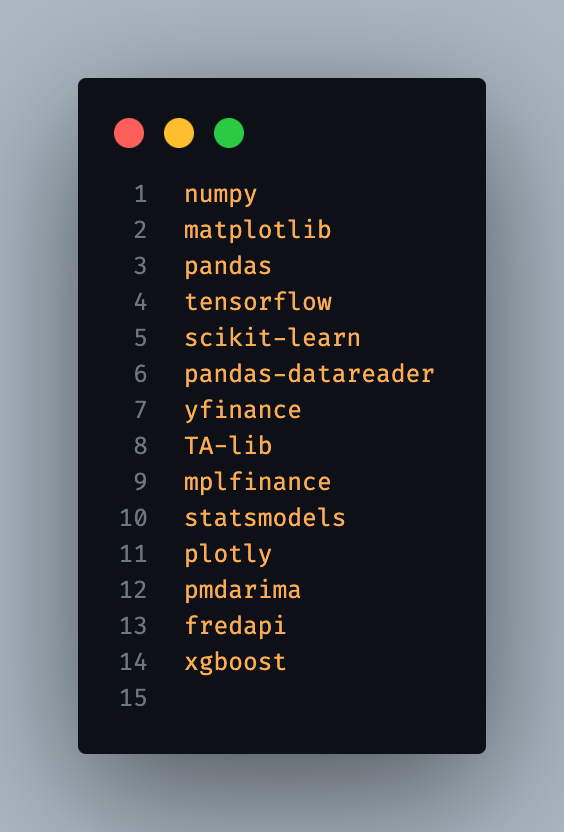
\includegraphics[width=8cm]{./images/requirements.png}
    \caption{Example of requirements.txt}
    \label{fig:requirements}
\end{figure}

\section{Understanding the Machine Learning 3}
\subsection{Exploring the required parameters for the ARIMA model}

\subsubsection{Codebase}

% TODO: Add Figure 3: Codebase for function to display the plots related to ARIMA parameters
\begin{figure}[ht]
    \centering
    % \includegraphics[width=0.8\textwidth]{figure3.png}
    \caption{Codebase for function to display the plots related to ARIMA parameters}
    \label{fig:arima_params_code}
\end{figure}

\subsubsection{Parameters}
\begin{itemize}
    \item \textbf{data: pandas.DataFrame}: The processed data that is used for finding the autoregressive order, difference order and moving average order.
\end{itemize}

\subsubsection{Functionalities}
In general, the given code will be used for plotting three graphs that correlate to three different essential parameters that the ARIMA model used, which are the number of lag observations in the model (p), the differencing degree to make the time series stationary (d), and the moving average order (q).

\begin{itemize}
    \item To observe the number of lags in the model (p), we will use the partial autocorrelation plot that is taken from \textbf{statsmodels} library and look for any crosses for the upper confidence interval, which is illustrated in the code and the plot below:
\end{itemize}

% TODO: Add Figure 4: Codebase used for plotting PACF
\begin{figure}[ht]
    \centering
    % \includegraphics[width=0.8\textwidth]{figure4.png}
    \caption{Codebase used for plotting PACF}
    \label{fig:pacf_code}
\end{figure}

% TODO: Add Figure 5: PACF Results of TSLA stock from 2015-01-01 and 2023-08-25
\begin{figure}[ht]
    \centering
    % \includegraphics[width=0.8\textwidth]{figure5.png}
    \caption{PACF Results of TSLA stock from 2015-01-01 and 2023-08-25}
    \label{fig:pacf_results}
\end{figure}

After a short investigation, we could see that first two lags have a significant correlation, which stays at 1 while the others stay around 0. Thus, a suggested p value that we obtained is 2.

To observe the moving average order (q), we will use the autocorrelation function plot that is also acquired from \textbf{statsmodels} library and look for any crosses for the upper confidence interval, which is illustrated in the code and the plot below:

% TODO: Add Figure 6: Codebase used for plotting ACF
\begin{figure}[ht]
    \centering
    % \includegraphics[width=0.8\textwidth]{figure6.png}
    \caption{Codebase used for plotting ACF}
    \label{fig:acf_code}
\end{figure}

% TODO: Add Figure 7: ACF Results of TSLA stock from 2015-01-01 and 2023-08-25
\begin{figure}[ht]
    \centering
    % \includegraphics[width=0.8\textwidth]{figure7.png}
    \caption{ACF Results of TSLA stock from 2015-01-01 and 2023-08-25}
    \label{fig:acf_results}
\end{figure}

The ACF plot points out that there is a significant autocorrelation at the first lag of the plot, thus suggests that the moving average order (q) is 1.

To observe the differencing degree (d), we will inspect the original time series of the stock price and its first and second time series differences.

% TODO: Add Figure 8: Codebase used for plotting time series
\begin{figure}[ht]
    \centering
    % \includegraphics[width=0.8\textwidth]{figure8.png}
    \caption{Codebase used for plotting time series}
    \label{fig:time_series_code}
\end{figure}

The given code above creates three subplots that sequently correlates to:
\begin{itemize}
    \item The original time series of the stock price.
    \item The first difference of the stock price's time series.
    \item The second difference of the stock price's time series.
\end{itemize}

% TODO: Add Figure 9: Time series differences of TSLA stock from 2015-01-01 and 2023-08-25
\begin{figure}[ht]
    \centering
    % \includegraphics[width=0.8\textwidth]{figure9.png}
    \caption{Time series differences of TSLA stock from 2015-01-01 and 2023-08-25}
    \label{fig:time_series_diff}
\end{figure}

Based on the given three plots, we could see that:
\begin{itemize}
    \item The original time series observed a clear upward trend, especially from 2020 onwards. This trend indicates that the series is non-stationary, which suggests that differencing is necessary to achieve stationarity.
    \item The first-order differencing of the original data appears much more stable compared to the original series plot. The mean seems to be roughly constant around zero, and the variance looks more consistent throughout the time period. This is a significant improvement in terms of stationarity.
    \item The second-order differencing doesn't seem to be a substantial improvement over the first-order differencing. Thus, might be introducing unnecessary complexity or noise into the data.
\end{itemize}

Therefore, first-order differencing (d=1) is sufficient to achieve stationarity in this time series.

\subsection{Function to create ARIMA model}

\subsubsection{Codebase}

% TODO: Add Figure 10: Codebase for function to create ARIMA model
\begin{figure}[ht]
    \centering
    % \includegraphics[width=0.8\textwidth]{figure10.png}
    \caption{Codebase for function to create ARIMA model}
    \label{fig:arima_model_code}
\end{figure}

\subsubsection{Parameters}
\begin{itemize}
    \item \textbf{train\_data: pd.DataFrame}: The training dataset that contains historical stock price data.
    \item \textbf{test\_data: pd.DataFrame}: The testing dataset that contains historical stock price data for evaluation.
    \item \textbf{p\_range: Tuple[int, int]}: The range of p (number of lag) values to consider in the ARIMA model. Default is (0, 5).
    \item \textbf{d\_range: Tuple[int, int]}: The range of d (differencing degree) values to consider in the ARIMA model. Default is (0, 2).
    \item \textbf{q\_range: Tuple[int, int]}: The range of q (moving average) values to consider in the ARIMA model. Default is (0, 5).
    \item \textbf{m: int}: The number of periods in each season for seasonal ARIMA. Default is 7.
    \item \textbf{seasonal: bool}: Whether to include seasonal components in the ARIMA model. Default is True.
\end{itemize}

\subsubsection{Functionalities}
In general, the major purpose of this function is to use the power of Auto Regressive Integrated Moving Average (ARIMA) model to predict the price of the stock based on the close price. The function performs the following steps:

\begin{itemize}
    \item \textbf{Data Extraction}: The function starts by extracting the value of the 'Close' price from both pre-processed train and test data, taken from the implemented \texttt{create\_dataset()} function.
    \item \textbf{Modelling and training the ARIMA}: Once the data has been processed, the function will call to the \texttt{auto\_arima()} function from the module \texttt{pmdarima} that helps creating the arima model with all of the required parameters and help selecting which model is the best parameters for the context. Specifically, the \texttt{auto\_arima()} function will consider the specified ranges for the required p, d, and q parameters, and seasonal components if required. Then, the function will perform trainings with different configurations to find out which model fits the best.
    \item \textbf{Model Summary}: Displays general informations of the selected ARIMA model, including the parameters and fit statistics.
    \item \textbf{Prediction}: Then, the function will perform some prediction based on the length of the test data to cover all of the periods on the test data.
    \item \textbf{Calculate Root Mean Square Error (RMSE)}: Once the prediction is finished, the function will calculate the Root Mean Square Error (RMSE) to indicate the error between the predicted values and the actual test data.
    \item \textbf{Return}: Finally, the function wil return an array that contains the predicted stock prices for the test period and the Root Mean Square Error of the predictions compared to the actual test data.
\end{itemize}

\subsection{Function to calculate the ensemble predictions}

\subsubsection{Codebase}

% TODO: Add Figure 11: Codebase for calculate the ensemble predictions
\begin{figure}[ht]
    \centering
    % \includegraphics[width=0.8\textwidth]{figure11.png}
    \caption{Codebase for calculate the ensemble predictions}
    \label{fig:ensemble_predictions_code}
\end{figure}

\subsubsection{Parameters}
\begin{itemize}
    \item \textbf{dl\_pred: np.ndarray}: The prediction results array from the deep learning model, could be from LSTM, GRU or RNN.
    \item \textbf{arima\_pred: np.ndarray}: The prediction results array from the ARIMA model.
    \item \textbf{dl\_rmse: float}: Root Mean Square Error (RMSE) value from the deep learning model predictions.
    \item \textbf{arima\_rmse: float}: Root Mean Square Error (RMSE) value from the ARIMA model predictions.
    \item \textbf{test\_data: pd.DataFrame | np.ndarray}: The actual test data for comparison and error calculation.
\end{itemize}

\subsubsection{Functionalities}
The purpose of this function is to create an ensemble prediction by combining the predictions from a deep learning model with an ARIMA model. The function performs the following procedures:

\begin{itemize}
    \item \textbf{Data Preparation}: Firstly, the function will flatten the deep learning predictions array if needed and starts modifying the length of predictions and test data to ensure they have the same size as different size of data could result in conflictions when working with charts and further calculations.
    \item \textbf{Performing ensemble prediction}: It then converts the deep learning predictions and the ARIMA predictions into a \texttt{numpy.array}, then sum all values from both arrays and divide it by 2 to get a unified ensemble prediction array.
    \item \textbf{Data cleaning}: Then, to ensure that the data is cleaned to perform a smooth plotting experience and for scalability, we search for NaN values in the test data and replace it with 0. Once the NaN values are replaced, the function prints the data after replacing NaN and if there are any NaN values in the deep learning and ARIMA prediction arrays.
    \item \textbf{Error Calculation}: Once the data is cleaned, the function will calculate the Root Mean Square Error (RMSE) for the ensemble predictions array and the average RMSE from both deep learning model predictions and the ARIMA predictions.
    \item \textbf{Return data}: Finally, the function will return ensemble predictions result as an \texttt{numpy.ndarray}, the Root Mean Square Error (RMSE) value for the ensemble predictions and the average RMSE value for both deep learning predictions and the ARIMA predictions.
\end{itemize}

\section{Deploying and Testing the Codebase}

\subsection{Codebase used for testing}
Please note that, since the given image below that shows the codebase for testing is too long, please refer to the file \texttt{main.py} for the full testing code.

% TODO: Add Figure 12: Codebase for testing
\begin{figure}[h]
    \centering
    % \includegraphics[width=0.8\textwidth]{figure12.png}
    \caption{Codebase for testing}
    \label{fig:testing_code}
\end{figure}

% Remember to include a bibliography section at the end of your document:

\bibliographystyle{plain}
\bibliography{references}


\end{document}
